\documentclass[11pt,a4paper]{article}
\usepackage[margin=2.3cm]{geometry}
\usepackage{amsmath,amssymb}
\usepackage{booktabs}
\usepackage{graphicx}
\graphicspath{{figures/}}
\usepackage{xcolor}
\usepackage[colorlinks=true,linkcolor=blue,urlcolor=blue,citecolor=blue]{hyperref}
\usepackage{siunitx}

% Default float parameters strand Table 2 + Fig 1 on a page that is a third
% whitespace. Let floats pack with text instead.
\renewcommand{\topfraction}{0.9}
\renewcommand{\bottomfraction}{0.8}
\renewcommand{\textfraction}{0.07}
\renewcommand{\floatpagefraction}{0.75}

\newcommand{\tauh}{\tau_{h}}
\newcommand{\tautau}{\tauh\tauh}
\newcommand{\mtautau}{m_{\tau\tau}}
\newcommand{\mvis}{m_{\mathrm{vis}}}
\newcommand{\mtau}{m_{\tau}}
\newcommand{\kl}{\kappa_{\lambda}}
\newcommand{\dR}{\Delta R}
\newcommand{\ptmiss}{p_{T}^{\mathrm{miss}}}
\newcommand{\yes}{\textcolor{teal}{$\checkmark$}}
\newcommand{\no}{\textcolor{red}{$\times$}}

\title{\vspace{-1.5cm}Delphes for HH$\rightarrow b\bar b\tau\tau$ NSBI:\\
\large full production tuned and validated against CMS}
\author{}
\date{\today}

\begin{document}
\maketitle
\vspace{-0.8cm}

\begin{abstract}
\noindent
The full Delphes production is tuned, ntuplised and validated: $3\times5$M signal events at
$\kl=0,1,5$ and $299$M $t\bar t$ events, $167\,$GB of analysis ntuples. In the
semi-leptonic channel --- the one the CMS NSBI result uses --- Delphes now reproduces CMS
to within a few percent in yield ($30\,491$ vs $28\,181$ at $\kl=0$) and agrees in shape on
$m_{HH}$, $m_{bb}$, $p_{T}^{HH}$, $\dR_{bb}$, $\Delta\phi_{HH}$, $p_{T}^{H1,H2}$,
$\cos\theta^{*}$, both $\tau$ $p_{T}$ and $\ptmiss$. Two things were found in the course of
this validation and are worth the PI's attention: the CMS lepton collections were being read
\emph{without} ID or isolation, which both broke the semi-leptonic comparison and biased the
lepton scale factors (Sec.~\ref{sec:leptons}); and the $b$-jet energy \emph{resolution} is
untuned by construction, only its scale (Sec.~\ref{sec:mbb}). One physics residual remains:
Delphes makes too many wide-angle $\tau$ pairs, visible as an excess at
$\dR_{\tau\tau}\simeq2.5$--$3.2$ and as high tails on $\mtautau$ and $\mvis$
(Sec.~\ref{sec:drtautau}). Since the last note the $t\bar t$ background has also been
compared against its own CMS anchor for the first time and the correction works
(Sec.~\ref{sec:ttbar}), and one new defect was found: FastMTT returns no solution for the
majority of events, because a Delphes $\tauh$ carries a jet mass far above $\mtau$
(Sec.~\ref{sec:fastmtt}).
\end{abstract}

\section{Where we stand}

\subsection{Production}

Everything downstream of Delphes: samples are never re-made, and every correction is a map
measured on a private CMS 2024 NanoAODv15 anchor and transferred. The anchor is the
\texttt{PowhegBugFix} campaign, the same one the Delphes signal samples were generated from.

\begin{table}[htbp]
\centering\small
\begin{tabular}{lrrl}
\toprule
sample & events & size & note \\
\midrule
signal $\kl=0,1,5$ & $3\times5.0$M & $7.3\,$GB & one \texttt{kl} column per event \\
$t\bar t$          & $298.7$M      & $160.2\,$GB & $1240/1244$ shards (Sec.~\ref{sec:shards}) \\
\midrule
total              & $313.7$M      & $167.5\,$GB & 33 parquet files \\
\bottomrule
\end{tabular}
\caption{Merged ntuples on \texttt{/ceph}. Produced by a 1394-job HTCondor campaign,
$22.4\,$min/job, $22.0\,$GB mean / $26.7\,$GB peak per job.\label{tab:production}}
\end{table}

The $\kl$ value is recorded per event. It is encoded only in the input path and the
ntuple schema had no field for it, so a merged signal sample would have been unusable for
NSBI --- the method is entirely about ratios \emph{between} $\kl$ hypotheses. It is now
recovered from the production plan at merge time and written as a column.

\subsection{Tuning}

\begin{table}[htbp]
\centering\small
\begin{tabular}{llp{6.3cm}}
\toprule
quantity & status & how \\
\midrule
b-tag efficiency ($b$, $c$, light) & \yes\ tuned & stochastic re-tag from \texttt{Jet.Flavor} at anchor UParT-AK4 Medium \\
b-jet energy \emph{scale}          & \yes\ tuned & inverted to unity against \texttt{GenJet} (self-anchored), $0.965$--$0.989$ \\
b-jet energy \emph{resolution}     & \no\ tuned  & not corrected at all --- Sec.~\ref{sec:mbb} \\
$\tauh$ ID efficiency              & \yes\ tuned & anchor \texttt{GenVisTau}$\rightarrow$DeepTau v2.5 Medium; includes HPS reco inefficiency \\
$\tauh$ energy response            & \yes\ tuned & \emph{distribution} resampled from anchor quantiles, not a median ratio \\
$\tauh$ visible mass               & \yes\ tuned & sampled per jet from anchor per-$p_{T}$ quantiles \\
$\ptmiss$ resolution               & \yes\ tuned & Gaussian smearing binned in jet $H_{T}$ \\
lepton reco efficiency             & \yes\ tuned & per-$p_{T}$ SFs, now $0.96$--$1.12$ ($e$), $1.03$--$1.07$ ($\mu$) \\
di-$\tau$ mass estimator           & \yes\ identical & same covariance-free FastMTT on both sides \\
\bottomrule
\end{tabular}
\caption{Object status. Every map is derived on the CMS anchor and applied downstream;
none needs a card change.\label{tab:tuning}}
\end{table}

The $\tauh$ energy correction is the one substantive change since the last note. A
multiplicative median scale factor cannot reshape a distribution, and the Delphes $\tau$
response carries a one-sided tail that CMS does not have (Fig.~\ref{fig:response}): at gen
$p_{T}=20$--$30\,\si{\GeV}$ one Delphes $\tau$ in ten had more than twice the median
response, against $1.08$ on CMS. The correction now samples the anchor response
\emph{distribution} per object, which reproduces the CMS response by construction and fixes
scale and width together. $\mvis$, $\tau_{1}\,p_{T}$, $\tau_{2}\,p_{T}$ and $\ptmiss$ all
overlay CMS after this change.

\begin{figure}[htbp]
\centering
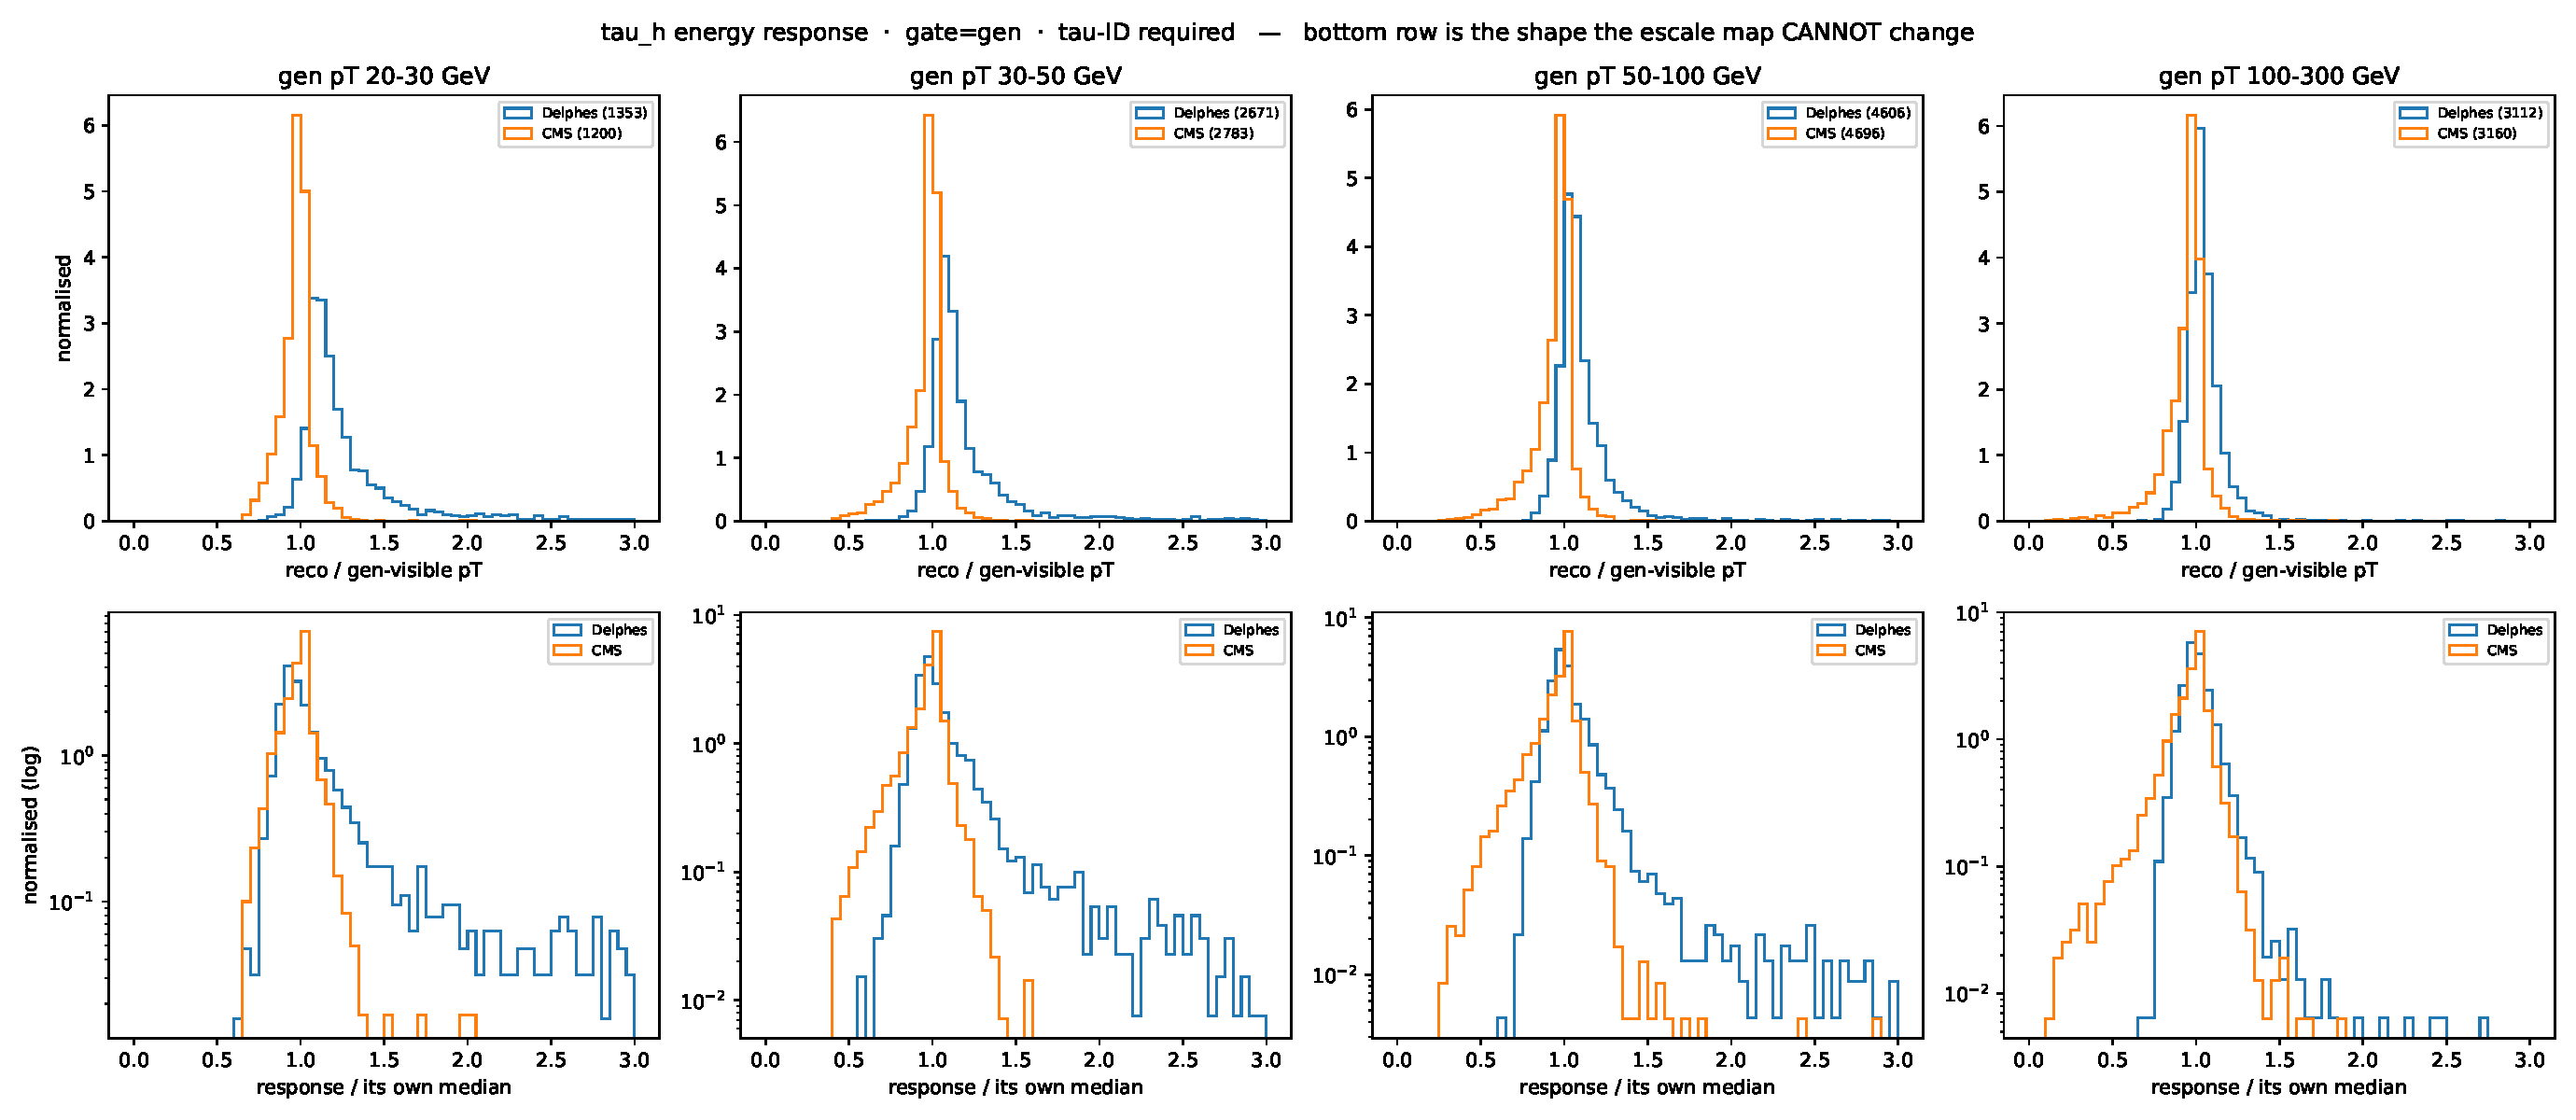
\includegraphics[width=\textwidth]{tau_response_id.pdf}
\caption{$\tauh$ energy response, Delphes vs the CMS anchor. The Delphes tail above the
median is what a multiplicative correction cannot remove and what motivated resampling the
distribution instead.\label{fig:response}}
\end{figure}

\section{Validation against CMS}

\subsection{The lepton definition --- a defect found and fixed}
\label{sec:leptons}

The CMS $\tau$-candidate pool was being built from the raw NanoAOD \texttt{Electron} and
\texttt{Muon} collections, with \emph{no} ID and no isolation requirement. Those collections
are loose enough to contain jet fakes that no analysis would use, whereas a Delphes lepton
has already passed the card's efficiency parameterisation, which is effectively an ID. The
two pools therefore did not mean the same thing, and the consequences were not cosmetic:

\begin{itemize}\itemsep1pt
\item CMS acquired candidates Delphes cannot produce --- $49\,950$ selected events against
      Delphes' $30\,491$ at $\kl=0$, a $1.6\times$ excess read at the time as a Delphes
      acceptance deficit.
\item A fake lepton paired with a real $\tau$ is back-to-back, so the CMS
      $\dR_{\tau\tau}$ and $\dR_{bb}$ distributions grew a spurious second peak at
      $\dR\simeq\pi$, plus $\mtautau$ and $\mvis$ tails and a flattened $\cos\theta^{*}$.
\item The same collections feed \texttt{lepton\_efficiency}, which sets the
      \texttt{electron\_sf} / \texttt{muon\_sf} anchor targets. The scale factors were
      therefore tuned toward loose-reco efficiency rather than toward analysis-quality
      leptons.
\end{itemize}

The cut is now applied in the NanoAOD \emph{reader}, so the tuning anchor and the validation
overlay cannot use different lepton definitions again, and a configured-but-missing ID
branch raises rather than silently reverting to the loose collection. Working points are
\texttt{Electron\_mvaIso\_WP80}, \texttt{Muon\_tightId} and
\texttt{Muon\_pfRelIso04\_all}${}<0.15$; \textbf{these should be checked against the CMS
$b\bar b\tau\tau$ baseline before anything is quoted.} After the fix the lepton fractions
match ($30\%$ Delphes vs $33\%$ CMS) and the scale factors sit near unity, which is itself
the evidence that the two definitions now agree --- against the loose collection they had to
make up a ${\sim}20\%$ gap.

\subsection{Result}

\begin{table}[htbp]
\centering\small
\begin{tabular}{lp{11.3cm}}
\toprule
\yes\ agree & $m_{HH}$ (the $\kl$ observable, at $\kl=0,1,5$); $m_{bb}$ peak;
$p_{T}^{HH}$; $\dR_{bb}$; $\Delta\phi_{HH}$; $p_{T}^{H1}$, $p_{T}^{H2}$;
$\cos\theta^{*}$; $\tau_{1}\,p_{T}$, $\tau_{2}\,p_{T}$; $\ptmiss$ \\
\midrule
\no\ disagree & $\dR_{\tau\tau}$ (Delphes excess at $2.5$--$3.2$), and the $\mtautau$ /
$\mvis$ high tails that follow from it; $m_{bb}$ \emph{width} \\
\bottomrule
\end{tabular}
\caption{NSBI inputs, semi-leptonic channel, 200k events per $\kl$ point against the
\texttt{PowhegBugFix} anchor including its \texttt{ext1} extension. Selected yields
Delphes/CMS: $30\,491/28\,181$ ($\kl=0$), $32\,783/31\,442$ ($\kl=1$), $24\,218/20\,443$
($\kl=5$).\label{tab:features}}
\end{table}

\subsection{The $t\bar t$ background}
\label{sec:ttbar}

The $t\bar t$ maps (\texttt{maps\_ttbar\_v1.json}) were applied to every $t\bar t$ event in
the production but had never been compared back against the anchor they came from. They now
have been, on \texttt{TTto2L2Nu} with the same selection on both sides, and the correction
works: the stock card over-produces $\tauh$ candidates by $1.68\times$ ($42\,293$ against
CMS' $25\,241$ in the same 200k events) and the re-tag brings that to $1.22\times$. Selected
yield moves from $0.70$ to $0.89$ of CMS.

All ten NSBI features agree in shape both before and after --- which is the part to read
carefully. The overlays are density-normalised, so a $1.68\times$ error in $\tauh$
\emph{rate} is invisible in them. Shape agreement is not evidence that the $\tauh$ object is
right, and the $22\%$ residual after tuning appears in no panel.

\section{Open items}

\subsection{$\dR_{\tau\tau}$: too many wide-angle $\tau$ pairs}
\label{sec:drtautau}

The one physics residual. Delphes has an excess at $\dR_{\tau\tau}\simeq2.5$--$3.2$, and
the $\mtautau$ and $\mvis$ high tails are probably the same events counted twice --- but
that is an inference, not a demonstration, so the argument is worth stating. For legs whose
masses are negligible against their energies,
$\mvis^{2}=2\,p_{T1}p_{T2}\,(\cosh\Delta\eta-\cos\Delta\phi)$ exactly, and both
angular terms grow monotonically as the pair separates; $\mtautau=\mvis/\sqrt{x_{1}x_{2}}$
inherits it. A wide pair is therefore a heavy pair --- though $\mvis$ is monotonic in
$\Delta\eta$ and $\Delta\phi$ separately and is \emph{not} a function of $\dR$ alone, so
``wide-angle'' rather than ``back-to-back'' is what $\dR$ measures. The converse does not
follow by itself: a heavy tail could equally come from harder $\tau$, since $\mvis$ also
grows with $p_{T1}p_{T2}$. What excludes that here is that $\tau_{1}\,p_{T}$ and
$\tau_{2}\,p_{T}$ both overlay CMS, leaving the angular term as the only place the excess
mass can come from. The direct test --- cutting $\dR_{\tau\tau}<2.5$ and asking whether the
$\mvis$ and $\mtautau$ tails go with it --- has not been run; if the tails survive, these
are two problems and not one. This matters for the feature set: dropping
$\dR_{\tau\tau}$ from the NSBI inputs would remove the most visible symptom while leaving
the identical artefact in $\mtautau$ and $\mvis$, which we certainly keep. The cause has to
be found rather than worked around.

The leading hypothesis is $\tauh$ mistag: a fake $\tau$ from the opposite hemisphere pairs
with a real one at $\dR\simeq\pi$. This is directly testable --- the overlay can split each
side into gen-matched and fake $\tau$ pairs and report the fake fraction --- and has not yet
been run at full statistics. The $t\bar t$ overlay (Sec.~\ref{sec:ttbar}) now supplies a first
measurement of the size of the effect: the stock card makes $1.68\times$ too many $\tauh$
candidates, so there is a real fake excess to account for. It is also actionable if
confirmed: the \texttt{tau\_fake\_response} map has its top three $p_{T}$ bins below the 200-entry
threshold and is borrowing them from neighbours, so the high-$p_{T}$ fake response is
extrapolated rather than measured.

\subsection{FastMTT returns no solution on the \emph{untuned} samples}
\label{sec:fastmtt}

Found while preparing the CROWN-matched ntuples, which are built from the \emph{untuned}
production. $\mtautau$, $m_{HH}$ and $p_{T}^{HH}$ taken from FastMTT are \texttt{NaN} on
$69\%$ of signal and $80\%$ of $t\bar t$ events there, while every other branch on those rows
is finite. The tuned arm does not have this failure, and the reason is worth stating
because it is the clearest example of a map earning its keep.

The mechanism is exact rather than statistical. The hadronic decay weight is non-zero only
for $x\ge(\mvis/\mtau)^{2}$, with $\mtau=1.777\,$GeV, so a leg whose visible mass exceeds
$\mtau$ has zero likelihood on the whole scan grid and the fit returns nothing. A Delphes
$\tauh$ \emph{is} an AK4 jet and carries the jet mass --- $5$--$15\,$GeV for a
$30$--$50\,$GeV jet, three to eight times $\mtau$, where a real HPS $\tauh$ never exceeds
the $a_{1}$ mass. Failures therefore track the $\tau$ jet mass rather than being a random
subset, which is why failing events have a higher visible $\mtautau$ ($92$ vs $72\,$GeV).

Two consequences. The elliptical signal region evaluates to \texttt{NaN} on those events and
rejects them, so it silently doubles as a FastMTT-success filter: a cut CMS quotes at $99\%$
signal efficiency runs at roughly $31\%$ here, on survivors biased in the very mass it
selects on. And the failure rate differs between processes ($69\%$ vs $80\%$), so on
the untuned samples FastMTT does not cancel between signal and background.

The tuning already fixes exactly this: the \texttt{tau\_mass} map redraws the $\tauh$
visible mass from the CMS anchor and hard-caps it at $1.70\,$GeV, just below $\mtau$, which
is the failure that map was written to remove. So this is a limitation of the untuned arm
rather than an open defect --- but the untuned arm is what the CROWN-matched NSBI inputs are
currently built from, so it bites in practice and those inputs should be regenerated from the
tuned production or have the cap applied. Two things remain genuinely open: the ellipse
should reject a failed fit \emph{explicitly} rather than through \texttt{NaN}$\rightarrow\infty$,
so the two rejection reasons are separable in a cutflow; and capping the mass leaves the
jet-level energy scale untouched, which only a $\tauh$ rebuild from the particle-flow
constituents would address.

\subsection{$m_{bb}$ width: the $b$-jet resolution is untuned}
\label{sec:mbb}

The $b$-jet correction inverts the response to unity against Delphes' \emph{own}
\texttt{GenJet}. That fixes the scale, does not touch the width, and never references CMS at
all. The $\tau$ side, by contrast, now has its full response distribution resampled from the
CMS anchor. $m_{bb}$ is therefore the feature receiving the weaker of the two treatments,
and its width does not match CMS.

The fix is the direct analogue of what worked for $\tau$: measure the CMS $b$-jet response
as a distribution and resample it. The machinery exists. The cost is the decision --- it
requires re-deriving the maps and re-running the full campaign ($\sim$10\,h) --- and it
should be validated on a subset before that is spent. Note also that the card runs without
pileup, so part of the CMS $b$-jet resolution has no counterpart in Delphes to correct.

\subsection{Four lost $t\bar t$ shards}
\label{sec:shards}

Four of 1244 $t\bar t$ shards ($0.3\%$) could not be produced: the dCache redirector
consistently routes those files to a pool node whose certificate does not cover the address
it hands out. Bounded retries were added and confirm the failure is deterministic, not
transient, so this is a site issue to report rather than a pipeline defect. Shards group
input files by size with no relation to physics, so the loss costs MC statistics and
introduces no bias; the shortfall is recorded in the merged manifest rather than hidden.

\section{Decisions and next steps}

\begin{enumerate}\itemsep2pt
\item \textbf{Confirm the lepton working points} against the CMS $b\bar b\tau\tau$ baseline.
      Everything downstream follows from them, and the current values are conventional
      choices rather than the analysis's.
\item \textbf{Clamp the $\tauh$ mass in FastMTT} (Sec.~\ref{sec:fastmtt}). One line, and
      it unblocks every $\mtautau$-based quantity; until it is in, use the visible mass.
\item \textbf{Run the gen-matched/fake split at full statistics} to test whether the
      $\dR_{\tau\tau}$ excess is $\tau$ mistag. Cheap, and it decides whether
      Sec.~\ref{sec:drtautau} is a fixable map problem or something deeper.
\item \textbf{Decide whether to tune the $b$-jet resolution} (Sec.~\ref{sec:mbb}). This is
      the only item costing a re-production, so it should be validated on a subset first.
\item \textbf{Then train.} The ntuples are ready and $\kl$-labelled; the feature set should
      be settled by measured $\kl$ separation and by training with and without candidate
      features, not by inspecting one-dimensional marginals.
\end{enumerate}

\section{Known limitations}
\label{sec:limits}

\emph{Accepted by design.} FastMTT is covariance-free and is run identically on both sides.
The cancellation argument
holds for the tuned samples, where \texttt{tau\_mass} keeps the $\tauh$ leg below $\mtau$. It
does \emph{not} hold for the untuned ones: Sec.~\ref{sec:fastmtt} shows the fit there fails at
different rates for signal and $t\bar t$, so the failures do not divide out and the visible
mass should be used instead. The card runs without pileup, so jet energy resolution is untuned and pileup jets
cannot exist; neither is fixable downstream. $\ptmiss$ smearing is now binned in jet $H_{T}$
but remains isotropic where the real resolution is anisotropic.

\emph{A scope bound, not a defect.} \texttt{tau\_mistag} is measured on the $b$-rich signal
anchor and fake rates are strongly jet-flavour dependent, so it is not valid for
fake-dominated backgrounds (QCD, W+jets). The present signal study is unaffected; a
background-heavy analysis would need those measured separately. There is likewise no CMS
anchor for DY, so DY cannot currently be tuned.

\emph{Untested --- risks, not accepted limitations.} The sampled $\tauh$ mass is drawn
independently of the $\tau$ energy and of the partner leg, whereas the true visible mass
correlates with decay mode; size unknown. Every map is flat-extrapolated above
$300\,\si{\GeV}$. That is probably benign here --- only ${\sim}2.8\%$ of b-jets exceed it,
the card's b-tag formula tends to a constant so flat is the right asymptote, and $\kl$
discrimination lives near threshold ($m_{HH}\simeq250$--$400\,\si{\GeV}$, where the triangle's
$s$-channel propagator makes the interference most $\kl$-sensitive) rather than in the
box-dominated tail. A boosted or high-$m_{HH}$ category would change that, by making the
extrapolated region the signal region.

\end{document}
